 \documentclass[oneside,12pt]{Classes/UFP}

%% Defina as propriedades do PDF gerado
\ifpdf
    \pdfinfo { /Title  (UFP THESIS)
               /Creator (TeX)
               /Producer (pdfTeX)
               /Author (Christophe Soares csoares@ufp.edu.pt)
               /CreationDate (D:20120101000000)  %format D:YYYYMMDDhhmmss
               /ModDate (D:20121101120000)
               /Subject (Como escrever uma tese em LaTeX)
               /Keywords (PhD, Thesis)}
    \pdfcatalog { /PageMode (/UseOutlines)
                  /OpenAction (fitbh)  }
\fi

% Titulo

\title{Thesis Template in \LaTeXe for \\ [1ex] % espaçamento
	Universidade Fernando Pessoa
}

\ifpdf
  \author{\href{mailto:csoares@ufp.edu.pt}{Christophe Soares}}
  \collegeordept{\href{http://fct.ufp.pt/t}{Faculdade de Ciências e Tecnologia}}
  \university{\href{http://www.ufp.pt}{Universidade Fernando Pessoa}}
% insert below the file name that contains the crest in-place of 'UnivShield'
  \crest{
\includegraphics[width=25mm]{UFP}}
\fi

\degree{Doctor of Philosophy / Master of Science}
\degreedate{Date to be defined}

% turn of those nasty overfull and underfull hboxes
\hbadness=10000
\hfuzz=50pt

% Put all the style files you want in the directory StyleFiles and usepackage like this:
\usepackage{StyleFiles/watermark}

% espaçamento de um e meio entre linhas
\onehalfspacing

\begin{document}

% defina a lingua do documento
%\language{english}


% Documento em fase de edição (comentar ou descomentar consoante precisar
\watermark{DRAFT COPY ONLY}


\maketitle

%set the number of sectioning levels that get number and appear in the contents
\setcounter{secnumdepth}{3}
\setcounter{tocdepth}{3}

\frontmatter % book mode only
\pagenumbering{roman}

% empty page
\newpage
\thispagestyle{empty}
\mbox{}


% Thesis Abstract -----------------------------------------------------


%\begin{abstractslong}    %uncommenting this line, gives a different abstract heading
\begin{abstracts}        %this creates the heading for the abstract page

This is where you write your abstract ...


\end{abstracts}
%\end{abstractlongs}



% Thesis Dedictation ---------------------------------------------------

\begin{dedication} %this creates the heading for the dedication page

I would like to dedicate this thesis to my loving parents ...

\end{dedication}

% Thesis Acknowledgements ------------------------------------------------


%\begin{acknowledgementslong} %uncommenting this line, gives a different acknowledgements heading
\begin{acknowledgements}      %this creates the heading for the acknowlegments


And I would like to acknowledge ...


\end{acknowledgements}
%\end{acknowledgmentslong}



\tableofcontents
\listoffigures
\listoftables
\printnomenclature  %% Print the nomenclature
\addcontentsline{toc}{chapter}{Nomenclature}

\mainmatter % book mode only
%%% Thesis Introduction --------------------------------------------------
\chapter{Introduction}
\ifpdf
    \graphicspath{{Introduction/IntroductionFigs/PNG/}{Introduction/IntroductionFigs/PDF/}{Introduction/IntroductionFigs/}}
\else
    \graphicspath{{Introduction/IntroductionFigs/EPS/}{Introduction/IntroductionFigs/}}
\fi

And this is how I would like to introduce my piece of work ...


Lorem ipsum dolor sit amet, consectetuer adipiscing elit, sed diam nonummy nibh euismod tincidunt ut laoreet dolore magna aliquam erat volutpat. Ut wisi enim ad minim veniam, quis nostrud exerci tation ullamcorper suscipit lobortis nisl ut aliquip ex ea commodo consequat. Duis autem vel eum iriure dolor in hendrerit in vulputate velit esse molestie consequat, vel illum dolore eu feugiat nulla facilisis at vero eros et accumsan et iusto odio dignissim qui blandit praesent luptatum zzril delenit augue duis dolore te feugait nulla facilisi. Nam liber tempor cum soluta nobis eleifend option congue nihil imperdiet doming id quod mazim placerat facer possim assum. Typi non habent claritatem insitam; est usus legentis in iis qui facit eorum claritatem. Investigationes demonstraverunt lectores legere me lius quod ii legunt saepius. Claritas est etiam processus dynamicus, qui sequitur mutationem consuetudium lectorum. Mirum est notare quam littera gothica, quam nunc putamus parum claram, anteposuerit litterarum formas humanitatis per seacula quarta decima et quinta decima. Eodem modo typi, qui nunc nobis videntur parum clari, fiant sollemnes in futurum.


% \pagebreak[4]
% \hspace*{1cm}
% \pagebreak[4]
% \hspace*{1cm}
% \pagebreak[4]

\chapter{My First Chapter But Note The Numbering ...}
\graphicspath{{Chapters/Chapter1/Chapter1Figs/PNG/}{Chapters/Chapter1/Chapter1Figs/PDF/}{Chapters/Chapter1/Chapter1Figs/}}

\section{First Paragraph}
And now I begin my first chapter here ...

Here is an equation\footnote{footnote test}:
\begin{eqnarray}
CIF: \hspace*{5mm}F_0^j(a) &=& \frac{1}{2\pi \iota} \oint_{\gamma} \frac{F_0^j(z)}{z - a} dz
\end{eqnarray}


\section{Second Paragraph}
and here I write more ...\cite{texbook}

\subsection{sub first paragraph}
... and some more ...

Now I would like to cite the following: \cite{latex} and \cite{texbook}
and \cite{Rud73}.

I would also like to include a picture ...

\begin{figure}[!htbp]
  \begin{center}
    \leavevmode
    \ifpdf
      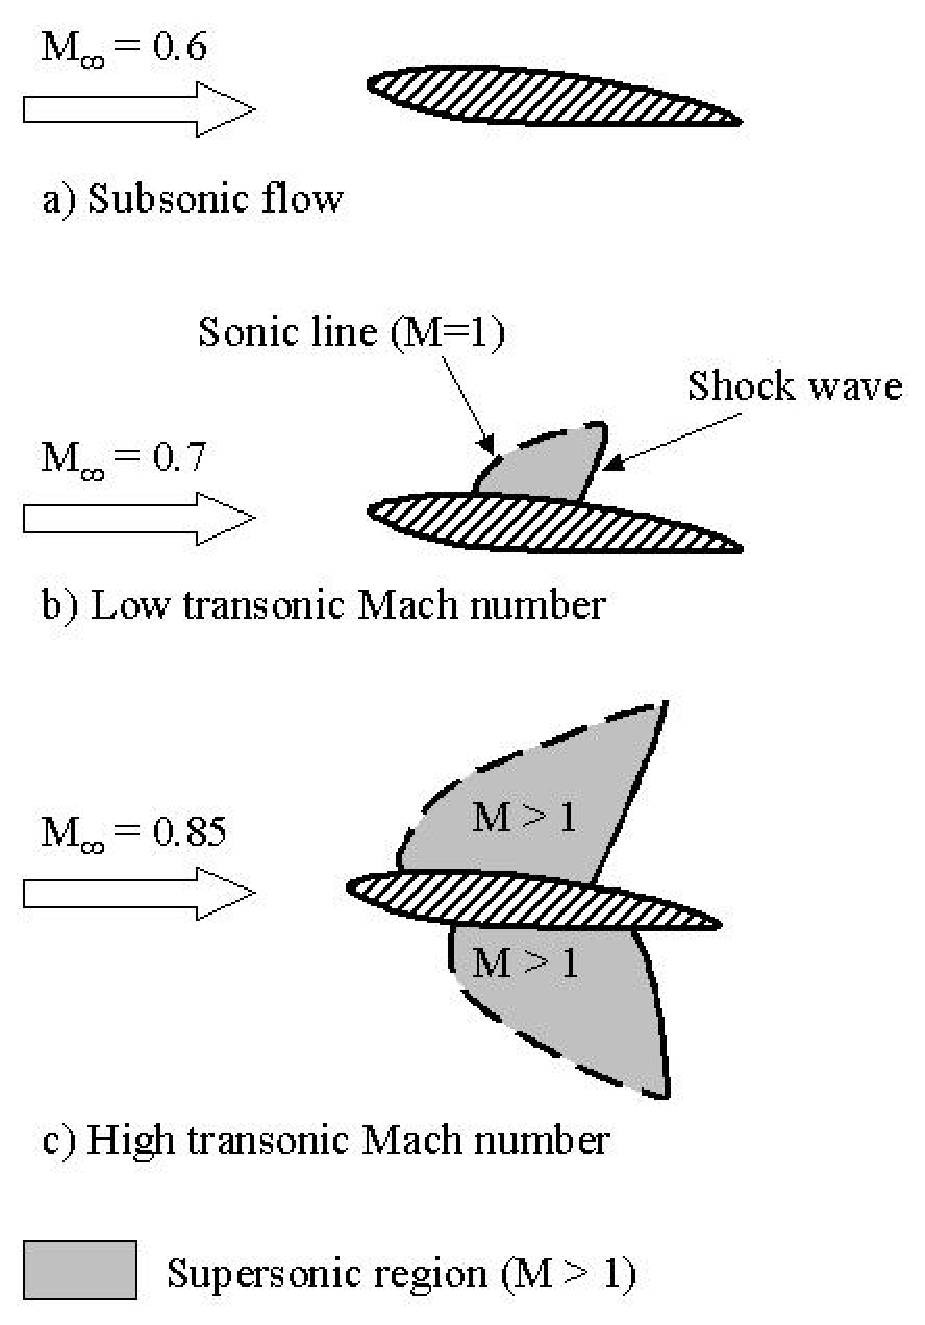
\includegraphics[height=6in]{aflow}
    \fi
    \caption{Airfoil Picture}
    \label{FigAir}
  \end{center}
\end{figure}

So as we have now labelled it we can reference it, like so (\ref{FigAir}) and it
is on Page \pageref{FigAir}. And as we can see, it is a very nice picture and we
can talk about it all we want and when we are tired we can move on to the next
chapter ...

I would also like to add an extra bookmark in acroread like so ...
\ifpdf
  \pdfbookmark[2]{bookmark text is here}{And this is what I want bookmarked}
\fi


\chapter{My Second Chapter}

\graphicspath{{Chapters/Chapter2/Chapter2Figs/PNG/}{Chapters/Chapter2/Chapter2Figs/PDF/}{Chapters/Chapter2/Chapter2Figs/}}

\section{First Section}
\markboth{\MakeUppercase{\thechapter. My Second Chapter }}
And now I begin my second chapter here ...

\begin{table}[tbh!]
\caption{Table} 
\label{tab:demo-1}
\centering
\begin{tabular}{l*{6}{c}r}
\hline
Team              & P & W & D & L & F  & A & Pts \\
\hline
FC Porto & 6 & 4 & 0 & 2 & 10 & 5 & 12  \\
Celtic            & 6 & 3 & 0 & 3 &  8 & 9 &  9  \\
FC Copenhagen           & 6 & 2 & 1 & 3 &  7 & 8 &  7  \\
SL Benfica     & 6 & 2 & 1 & 3 &  5 & 8 &  7  \\
\end{tabular}
\end{table}

\section{Second Section}
\markboth{\MakeUppercase{\thechapter. My Second Chapter }}
And here I write more ...

\subsection{first subsection in the Second Section}
... and some more ...

\subsection{second subsection in the Second Section}
... and some more ...

\subsection{third subsection in the Second Section}
... and some more ...

\chapter{My Third Chapter}

\graphicspath{{Chapters/Chapter3/Chapter3Figs/PNG/}{Chapters/Chapter3/Chapter3Figs/PDF/}{Chapters/Chapter3/Chapter3Figs/}}


\section{First Section of the Third Chapter}
\markboth{\MakeUppercase{\thechapter. My Third Chapter }}{\thechapter. My Third Chapter}

And now I begin my third chapter here ...

\subsection{first subsection in the First Section}
... and some more 

\subsection{second subsection in the First Section}
... and some more ...

\subsubsection{first subsub section in the second subsection}
... and some more in the first subsub section otherwise it all looks the same
doesn't it? well we can add some text to it ...

\subsection{third subsection in the First Section}
... and some more ...

\subsubsection{first subsub section in the third subsection}
... and some more in the first subsub section otherwise it all looks the same
doesn't it? well we can add some text to it and some more and some more and
some more and some more and some more and some more and some more ...

\subsubsection{second subsub section in the third subsection}
... and some more in the first subsub section otherwise it all looks the same
doesn't it? well we can add some text to it ...

\section{Second Section of the Third Chapter}
\markboth{\MakeUppercase{\thechapter. My Third Chapter }}{\thechapter. My Third Chapter}
A	nd here I write more ...

\def\baselinestretch{1}
\chapter{My Conclusions ...}

\graphicspath{{Chapters/Conclusions/ConclusionsFigs/PNG/}{Chapters/Conclusions/ConclusionsFigs/PDF/}{Chapters/Conclusions/ConclusionsFigs/}}


\def\baselinestretch{1.66}

Here I put my conclusions ...


\backmatter % book mode only
\appendix
\chapter{Appdx A}

and here I put a bit of postamble ...


\chapter{Appdx B}

and here I put some more postamble ...



%escolha um dos 3 estilos de bibliografia
\bibliographystyle{plainnat}
%\bibliographystyle{Classes/UFPbib}
%\bibliographystyle{Classes/jmb} % bibliography style

\renewcommand{\bibname}{References} 	% personalizar o nome da secção das referências bibliográficas
\bibliography{References/references} 		% Caminho para o bibtex

\end{document}
